\chapter{CMS detector and LHC}
This analysis is done by using the data recorded by the Compact Muon Solenoid(CMS) detector at Large Hadron Collider(LHC). CMS is one of the two biggest experiments in LHC, and is involed in the discovery of Higgs boson in July, 2011. In this chapter, the brief overveiw of LHC and CMS detector will be introduced.

\section{Large Hadron Collider} 
The LHC is the biggest particle accelerator that humen ever build on earth. The construction of the LHC start from 1998 and end up in 2008. Fig. \ref{fig:LHC} shows the overview of LHC. The LHC is designed to have 27 km in circumference lies in a ring tunnel hundred meters underground acrossing French-Swiss border. It is a proton-proton collider. The designed top collision energy is 14 TeV and can afford luminosity up to $10^{-34} cm^{-2}s^{-1}$. Few days after its first operation in November 2009, the center-of-mass energy per beam reached 1.18 TeV, break the record held by Tevatron in Fermilab becoming the most powerful particle accelerator in world till today.     
\newline There are four collsion points at LHC, corresponding to four main experiments. They are CMS, ATLAS, ALICE, and LHCb respectively. The ALICE and the LHCb experiments are for specify studies. The ALICE experiment put the sight on heavy ion collisions, learning the matters in high density conditions. The LHCb experiment aim tofind the clues of matters and anti-matters' mystery by observing the production and decay of b quarks. Last, the CMS and the ATLAS are the two biggest experiments at LHC, and their detector design are for general purpose. They involved in any kind of search in high energy physics, such as SUSY, dark matter, or other exotica particles, and most importantly, the discovery of Higgs boson in July, 2012.  

\begin{figure}
 \begin{center}
  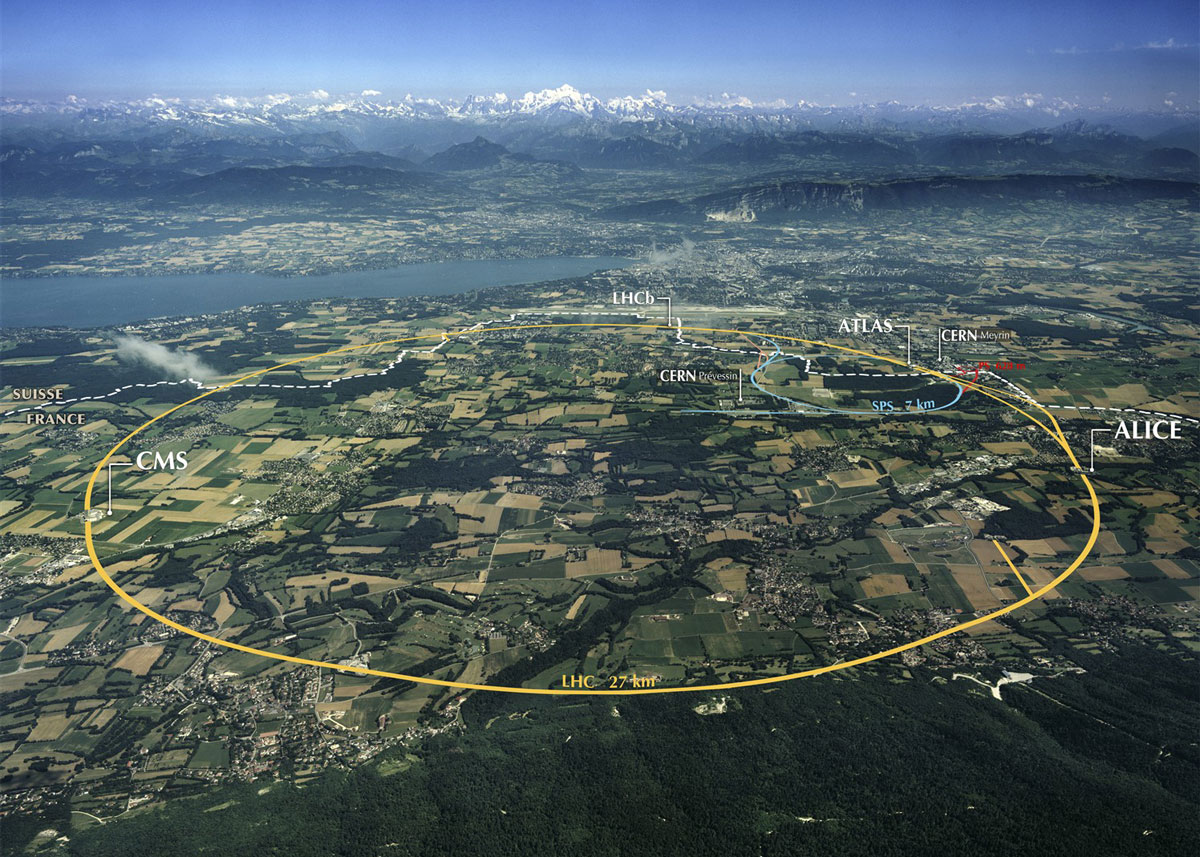
\includegraphics[width=\textwidth]{plot/cern-lhc-aerial.jpg}
 \end{center}
\caption{\label{fig:LHC}The Large Hadron Collider.}
\end{figure}

\section{CMS detector}
The design of CMS has to satisfy the requirements below to make it a discovery machine. 

\begin{itemize}
\item Good muon identification and momentum resolution over a wide range of momenta in the region $|\eta| < 2.5$, good dimuon mass resolution, and the ability to determine unambiguously the charge of muons at high momentum.
\item Good charged particle momentum resolution and reconstruction efficiency in the inner tracker.
\item Good electromagnetic energy resolution, good diphoton and dielectron mass resolution, wide geometric coverage ($|\eta| < 2.5$), measurement of the direction of photons and/or correct localization of the primary interaction vertex, $\pi^{0}$ rejection and efficient photon and lepton isolation at high luminosities.
\item Good Missing transverse energy and dijet mass resolution.
\end{itemize}

The construction, installation and commissioning of CMS is progressing well, though not
without challenges, towards the goal of being ready for collisions in the second half of 2007.
The overall layout of CMS is shown in Fig. \ref{fig:CMS}. The core of CMS sits a 13-m-long, 5.9 m
inner diameter superconducting solenoid, providing magnetic field up to 4 tesla. There are 4 sub-detector sets in CMS. The most inner part is occupied by tracking system composed of silicon pixel and strips. Behind the tracker, there sits the electromagnetic calorimeter(ECAL), and the hadron calorimeter(HCAL). At exterior most of the CMS, the muon chambers are arranged in this part. Due to the muon chambers are outside the magnet, there are layers of steel serve as return yoke in between each set of muon chambers. The overall dimensions of the CMS detector are a length of 21.6 m, a diameter of 14.6 m and a total weight of 12500 tons.

\begin{figure}
 \begin{center}
  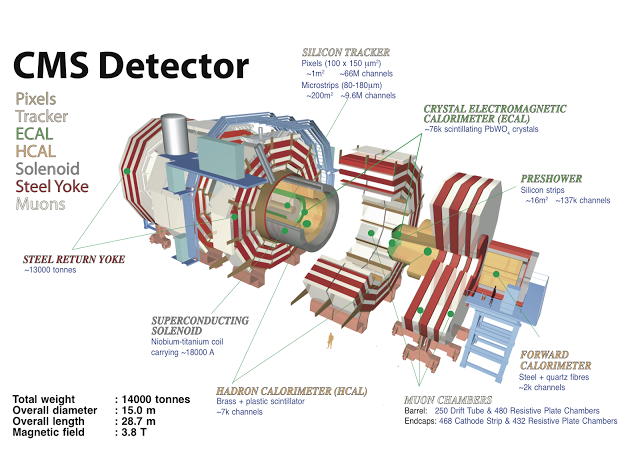
\includegraphics[width=0.9\textwidth]{plot/cms_3d_jul10.png}
 \end{center}
\caption{\label{fig:CMS}The Compact Muon Solenoid.}
\end{figure}

\subsection{Coordinate in CMS}
The coordinate system adopted by CMS has the origin centered at the nominal collision point
inside the experiment, the y-axis pointing vertically upward, and the x-axis pointing radially inward toward the center of the LHC. Thus, the z-axis points along the counter-clockwise beam direction. The azimuthal angle $\phi$ is measured from the x-axis in the x-y plane. The polar angle $\theta$ is measured from the z-axis. Pseudorapidity is
defined as $\eta = -ln tan(\theta /2)$. Thus, the momentum and energy measured transverse to the
beam direction, denoted by $p_{T}$ and $E_{T}$ , respectively, are computed from the x and y components. The imbalance of energy measured in the transverse plane is denoted by $E_{T}^{miss}$.

\subsection{Superconduction solenoid}
CMS chose a large superconducting solenoid, the parameters of which are given in Tab \ref{tab:magnet}. A large bending power can be obtained for a modestly-sized solenoid, albeit a high-field superconducting one, as the bending starts at the primary vertex. A favorable length to radius ratio is necessary to ensure good momentum resolution in the forward region as well.
\newline The main features of the CMS solenoid are the use of a high-purity aluminium-stabilised
conductor and indirect cooling (by thermosyphon), together with full epoxy impregnation.
This technique was successfully used previously in the construction of the large solenoids for
ALEPH and DELPHI at LEP and for H1 at HERA. However, the large increase in magnetic field, Ampere-turns, forces and stored energy (2.7 GJ) necessitated
changes. In particular, a four-layer winding has been adopted using a novel conductor with a
larger cross-section that can withstand an outward pressure (hoop stress) of 64 atmospheres.
The conductor carries a current of 20 kA and has a compound structure. The Rutherford-type
cable is co-extruded with pure aluminium, which acts as a thermal stabiliser. This insert is
then electron-beam-welded to 2 plates, made of a high-strength aluminium alloy, for the
mechanical reinforcement. The overall conductor cross section is 64$\times$22 $mm^{2}$.

\begin{table}[h]
 \begin{center}
  \begin{tabular}{|l|c|}
\hline
Field & 4T \\
\hline
Inner Bore & 5.9 m \\
\hline
Length & 12.9 m \\
\hline
Number of Turns & 2168 \\
\hline
Current & 19.5 kA \\
\hline
Stored energy & 2.7 GJ \\
\hline
Hoop stress & 64 atm \\
\hline
\end{tabular}
\caption{\label{tab:magnet} Parameters of the CMS superconducting solenoid.}
\end{center}
\end{table}

\subsection{Tracking system}
Tracking system is the first detector setup that the productions of collisions first contacted. This part of sub-detecter trace the charged particles' trajectories without consuming their energy(at least as possible), helping physics to find out the vertex and momentum of each particle by linking the tracks to the collider's pipe and measuring the curves of particles under 4 T magnetic field. 
\newline The layout of the CMS tracker is shown in Fig. \ref{fig:tracker}. The outer radius of the CMS tracker
extends to nearly 110 cm, and its total length is approximately 540 cm. The tracker in CMS is made of silicon pixel and silicon strip. Close to the interaction vertex, the pixel detector stands here to improve the vertex resolution. Pixel detecter consists of 3 barrel layers with 2 endcap disks on each side on them(Fig. \ref{fig:pixel}). The 3 barrel layers are located at mean radii of 4.4 cm, 7.3 cm and 10.2 cm, and have a length
of 53 cm. The 2 end disks, extending from 6 to 15 cm in radius, are placed on each side at
|z| = 34.5 cm and 46.5 cm. The spatial resolution is measured to be about 10 $\mu m$ for the $r-\phi$ measurement and about
20 $\mu m$ for the z measurement. 
\newline Outside the pixel tracker, there comes the tracker composed of strips. The barrel part is separated into an
Inner(TIB) and an Outer Barrel(TOB). In order to avoid excessively shallow track crossing angles, the
Inner Barrel is shorterthan the Outer Barrel. The TIB is made of 4 layers and covers up to $|z| < 65 cm$, using
silicon sensors with a thickness of 320 $\mu m$ and a strip pitch which varies from 80 to 120 $\mu m$. The TOB
comprises 6 layers with a half-length of $|z| < 110 cm$. The endcaps are divided into the TEC (Tracker End Cap) and TID (Tracker Inner Disks).
Each TEC comprises 9 disks that extend into the region $120 cm< |z| < 280 cm$, and each
TID comprises 3 small disks that filt he gap between the TIB and the TEC. The entire silicon stripdetector consists of almost 15400 modules, which will be mounted on
carbon-fir rstructures and housed inside a temperature controlled outer support tube. The
operating temperature will be around -$\degree C$. 

\begin{figure}
 \begin{center}
  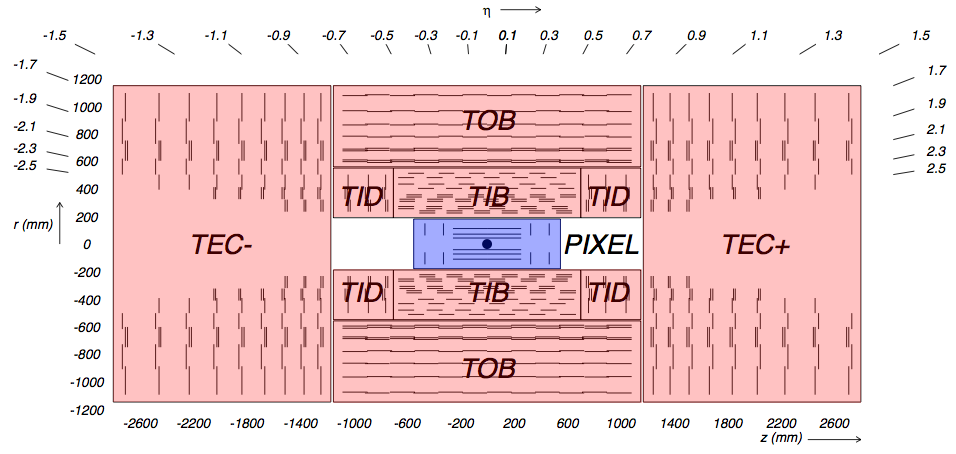
\includegraphics[width=\textwidth]{plot/tracker.png}
 \end{center}
\caption{\label{fig:tracker}The tracker layout of CMS.}
\end{figure}

\begin{figure}
 \begin{center}
  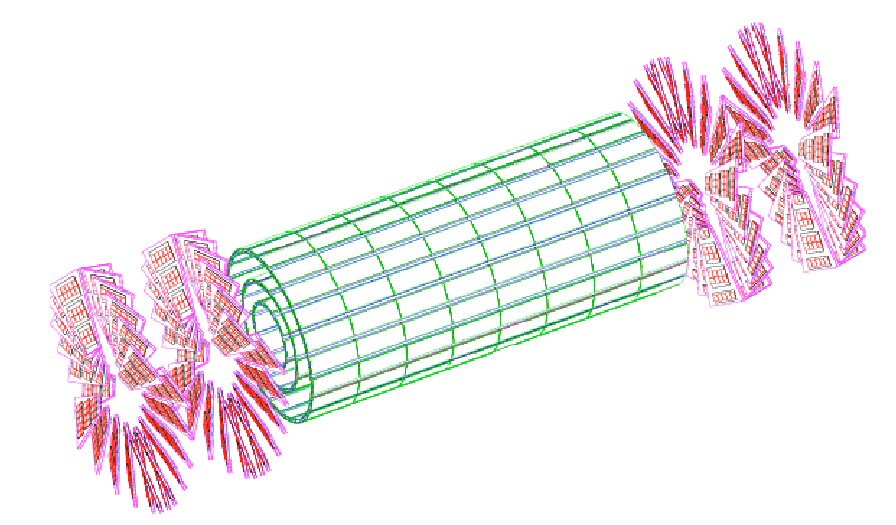
\includegraphics[width=0.6\textwidth]{plot/pixel.png}
 \end{center}
\caption{\label{fig:pixel}Pixel detector inside tracker.}
\end{figure}

\subsection{Electromagmetic calorimeter}
High energy electrons and photons interact with matter mainly through bremsstrahlung and electron-positron
pair production, depositing practically all their energy in an adequately designed calorimeter. Lead tungstate
crystals (PbWO$_{4}$) have been chosen as the material for the CMS electromagnetic calorimeter (ECAL) for two
reasons. Firstly, they are dense, so that an electromagnetic shower develops early and is very likely fully contained
within a compact device. Secondly, they are fast scintillators, providing the possibility to detect the light emitted
in the showering process. Silicon avalanche photo diodes (APD) have been selected for the light readout in the
central region, since these devices can operate in a hostile radiation environment and high magnetic field.
\newline The barrel section (EB) has an inner radius of 129 cm. It is structured as 36 identical supermodules,
each covering half the barrel length and corresponding to a pseudorapidity
interval of $0 < |\eta| < 1.479$. The endcaps (EE), at a distance of 314 cm from the vertex and covering a pseudorapidity
range of $1.479 < |\eta| < 3.0$, are each consisting of semi-circular aluminium
plates from which are cantilevered structural units of 5$\times$5 crystals, known as supercrystals. A preshower
device is placed in front of the crystal calorimeter over much of the endcap pseudorapidity
range. The active elements of this device are 2 planes of silicon strip detectors, with a pitch
of 1.9 mm, which lie behind disks of lead absorber at depths of 2 $X_{0}$ and 3 $X_{0}$.
Beam tests have shown that the energy resolution of ECAL modules is excellent.

\subsection{Hadron calorimeter}
Hadrons such as protons, neutrons, pions or Kaons are strongly interacting particles, which feel the force that
binds nuclei together. Like for electrons or photons their energy and position can be measured in a calorimeter.
Hadronic showers start to develop later and have larger longitudinal and lateral dimensions than electromagnetic
ones. The HCAL is made of alternating plates of brass and plastic scintillator read out through wavelength shifting optical fibres by
photosensors in the barrel and endcap regions. The photosensors are hybrid photodiodes, which consist of a fibre-optic entrance window onto which a photocathode is deposited, followed by a gap of several millimeters over which a large applied electric field accelerates photoelectrons onto a silicon diode target. The very forward
part of HCAL, the HF located at both sides of the detector, has steel absorber plates sampled by quartz fibres due to their good radiation tolerance.

\subsection{Muon chamber}
In order to detect a passing muon, three different types of muon chambers form a system consisting of drift tube
(DT) chambers in the barrel, cathode strip chambers (CSC) in the endcaps and resistive plate chambers (RPC)
glued to the DT and CSC chambers. Four layers, also called stations, of DT/RPC and CSC/RPC chambers are
embedded into the iron yoke in order to make up a redundant system that can guarantee optimal performance
both in the reconstruction of tracks and in triggering. The layout of one quarter of the CMS muon system for initial low luminosity running is
shown in Fig. \ref{fig:muonchamber}. In the Muon Barrel (MB) region, 4 stations of detectors are arranged in
cylinders interleaved with the iron yoke. In each of the endcaps, the CSCs and RPCs are arranged in 4 disks perpendicular to
the beam, and in concentric rings, 3 rings in the innermost station, and 2 in the others.

\begin{figure}
 \begin{center}
  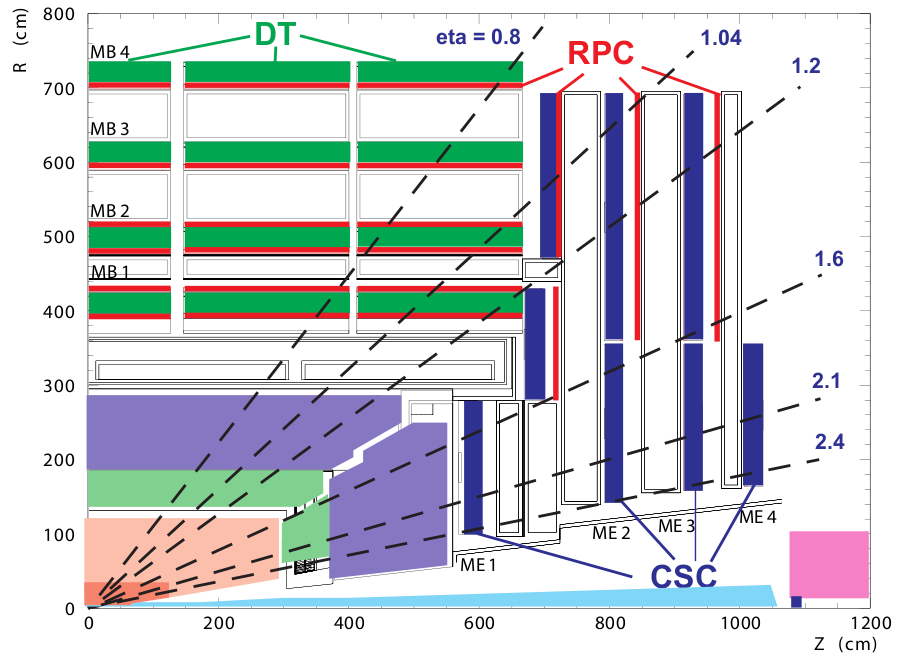
\includegraphics[width=0.9\textwidth]{plot/muonchamber.png}
 \end{center}
\caption{\label{fig:muonchamber}The layout of muon chambers in CMS.}
\end{figure}

\subsection*{Drift tube chamber}
The drift tube (DT) system measures muon positions in the barrel part of the detector. Each 4-cm-wide tube contains a stretched wire within a gas volume. When a muon or any charged particle passes through the volume it knocks electrons off the atoms of the gas. These follow the electric field ending up at the positively-charged wire.
The Barrel Detector consists of 250 chambers organized in 4 layers (stations labeled MB1, MB2, MB3 and MB4 with the
last being the outermost) inside the magnet return yoke, at radii of approximately 4.0, 4.9, 5.9 and 7.0 m from the beam axis.
Chambers in different stations are staggered so that a high-$p_{T}$ muon produced near a sector boundary crosses at least 3 out of
the 4 stations. There are 12 chambers in each of the 3 inner layers. In the 4th layer, the top
and bottom sectors host 2 chambers each, thus leading to a total of 14 chambers per wheel
in this outermost layer. The maximum drift length is 2.0 cm and the single-point resolution is about 200 $\mu m$. Each station is designed to give a muon vector in space, with a
$\phi$ precision better than 100 $\mu m$ in position and approximately 1 mrad in direction.
\newline Each DT chamber has 1 or 2 RPCs coupled to it before installation, depending on the station.
In stations MB1 and MB2, each package consists of 1 DT chamber sandwiched between 2
RPCs. In stations MB3 and MB4, each package comprises 1 DT chamber and 1 RPC, which
is placed on the innermost side of the station. A high-$p_{T}$ muon thus crosses up to 6 RPCs
and 4 DT chambers, producing up to 44 measured points in the DT system from which a
muon-track candidate can be built.

\subsection*{Cathode strip chamber}
The Muon Endcap (ME) system comprises 468 CSCs in the 2 endcaps.
Each CSC is trapezoidal in shape and consists of 6 gas
gaps, each gap having a plane of radial cathode strips and a plane of anode wires running
almost perpendicularly to the strips. All CSCs except those in the third ring of the first endcap disk (ME1/3) are overlapped in phi to avoid gaps in the muon acceptance. The gas ionization
and subsequent electron avalanche caused by a charged particle traversing each plane of a
chamber produces a charge on the anode wire and an image charge on a group of cathode
strips. The signal on the wires is fast and is used in the Level-1 Trigger. However, it leads to
a coarser position resolution. A precise position measurement is made by determining the
centre-of-gravity of the charge distribution induced on the cathode strips. The spatial resolution provided by each chamber
from the strips is typically about 200 $\mu m$ (100 $\mu m$ for ME1/1). The angular resolution in $\phi$ is
of order 10 mrad.

\subsection*{Resistive plate chamber}
Resistive plate chambers (RPC) are fast gaseous detectors that provide a muon trigger system parallel with those of the DTs and CSCs.
RPCs consist of two parallel plates, a positively-charged anode and a negatively-charged cathode, both made of a very high resistivity plastic material and separated by a gas volume.
When a muon passes through the chamber, electrons are knocked out of gas atoms. These electrons in turn hit other atoms causing an avalanche of electrons. The electrodes are transparent to the signal (the electrons), which are instead picked up by external metallic strips after a small but precise time delay. The pattern of hit strips gives a quick measure of the muon momentum, which is then used by the trigger to make immediate decisions about whether the data are worth keeping. RPCs combine a good spatial resolution with a time resolution of just 1 ns.

\section{Trigger system}
The LHC accelerator will provide proton-proton and heavy-ion collisions at high interaction rates. The bunch
crossing interval for protons is 25 ns. Depending on luminosity, several proton-proton interactions occur at each
crossing of the beams. At the nominal design luminosity of $10^{-34} cm^{-2}s^{-1}$ approximately 20 proton-proton events
are superimposed, and the interaction rate is of the order of 1 GHz. Since it is impossible to store and process
the large amount of information. About 1 MB of zero-suppressed data per event associated with the resulting
high number of events, a drastic rate reduction has to be achieved. This task is performed by the trigger system,
which is the start of the physics event selection process. In CMS the input rate is reduced in two steps called
Level-1 Trigger(L1T) and High-Level Trigger(HLT), respectively. The structure of the trigger system is shown in Fig. \ref{fig:trigger}.  

\begin{figure}
 \begin{center}
  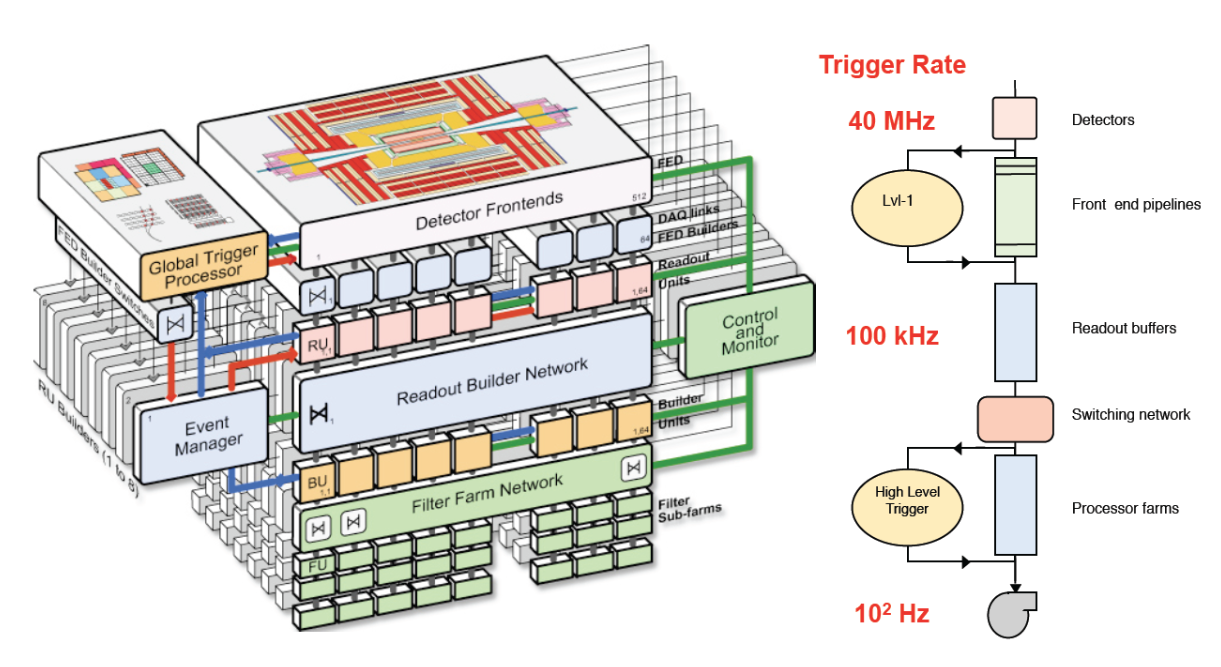
\includegraphics[width=0.9\textwidth]{plot/trigger.png}
 \end{center}
\caption{\label{fig:trigger}The trigger system in CMS.}
\end{figure}

\subsection*{Level-1 trigger}
The size of the LHC detectors and the underground caverns imposes a minimum transit time
for signals from the front-end electronics to reach the services cavern housing the Level-1
trigger logic and return back to the detector front-end electronics. The total time allocated for
the transit and for reaching a decision to keep or discard data from a particular beam crossing
is 3.2 $\mu s$. During this time, the detector data must be held in buffers while trigger data is
collected from the front-end electronics and decisions reached that discard a large fraction of
events while retaining the small fraction of interactions of interest.
Of the total latency, the time allocated to Level-1 trigger calculations is less than 1 $\mu s$.
\newline The Level-1 triggers involve the calorimetry and muon systems, as well as some correlation of information between these
systems. The Level-1 decision is based on the presence of “trigger primitive” objects such
as photons, electrons, muons, and jets above set $E_{T}$ or $p_{T}$ thresholds. It also employs global
sums of $E_{T}$ and $E_{T}^{miss}$. During the Level-1 decision-making period, all the high-resolution data is held in pipelined
memories. Commodity computer processors make subsequent decisions using more detailed information from all of the detectors in more and more sophisticated algorithms that
approach the quality of final reconstruction.
 
\subsection*{High level trigger}
Through the event building ``switch'', data from
a given event are transferred to a processor. Each processor runs the same high-level trigger
(HLT) software code to reduce the Level-1 output rate of 100 kHz to 100 Hz for mass storage.
Various strategies guide the development of the HLT code. Rather than reconstruct all possible objects in an event, whenever possible only those objects and regions of the detector that
are actually needed are reconstructed.

